\RequirePackage{fix-cm}
%
\documentclass{svjour3}                     % onecolumn (standard format)
%\documentclass[smallcondensed]{svjour3}     % onecolumn (ditto)
%\documentclass[smallextended]{svjour3}       % onecolumn (second format)
%\documentclass[twocolumn]{svjour3}          % twocolumn


\usepackage{graphicx}
\usepackage{amsmath}
\usepackage{amsfonts}
\usepackage{amssymb}
\usepackage{natbib}
\usepackage{algorithm}
\usepackage{algpseudocode}

\journalname{Journal of Geodesy}
\begin{document}

\title{Unbiased characterization of noise in geodetic data}
\titlerunning{Unbiased noise characterization}        % if too long for running head
\author{Trever T. Hines \and Eric A. Hetland}
%\authorrunning{Short form of author list} % if too long for running head

\institute{Trever T. Hines \at
           Department of Earth and Environmental Sciences \\
           University of Michigan, Ann Arbor \\
           Ann Arbor, MI, USA \\
           \email{hinest@umich.edu}  \\
           \and
           Eric A. Hetland \at
           Department of Earth and Environmental Sciences \\
           University of Michigan, Ann Arbor \\
           Ann Arbor, MI, USA \\
           \email{ehetland@umich.edu}
}

\date{Received: date / Accepted: date}
% The correct dates will be entered by the editor

\maketitle

\begin{abstract}
Geodetic time series contain temporally correlated noise that must be quantified before the data can be used to make geophysical inferences. If the noise is not accurately quantified then there is a risk of underestimating the uncertainties on inferred geophysical parameters. The maximum likelihood estimation (MLE) method is commonly used to characterize noise in geodetic time series; however, this method is known to be biased. Specifically, the MLE method has a tendency to underestimate the amplitude of random walk noise. This bias is most pronounced when estimating the noise in shorter time series. We discuss an unbiased alternative to the MLE method, which is known as the restricted maximum likelihood (REML) method. We use synthetic tests to demonstrate that the REML method does not suffer from the bias inherent in the MLE method. Since the computational costs of the REML and MLE method are nearly equivalent, the REML method should always be prefered over the MLE method when quantifying noise in geodetic data. 

\keywords{Keyword1 \and Keyword2}
\end{abstract}

\section{Introduction}\label{sec:Introduction}
Before geodetic data can be used to make geophysical inferences, it is necessary to have an accurate noise model. Here we consider noise to be any observed deformation that is not representative of the cohesive crustal block. The noise in geodetic time series is temporally correlated and its power spectrum can often be described by a power law relationship \citep{Agnew1992},       
\begin{equation}\label{eq.PowerLaw}
  P(f) = P_o f^{-k},
\end{equation}
where $f$ is frequency, $k$ is the spectral index and $P_o$ is the noise amplitude. For data recorded by strain and tilt meters \citep{Wyatt1982,Wyatt1989} and electronic distance measuring (EDM) instruments \citep{Langbein1997}, the temporally correlated noise can be modeled as a random walk ($k = 2$). In these studies, the random walk noise was attributed to unstable geodetic monuments. Global Positioning System (GPS) data, which is prone to additional non-physical sources of error, often has temporally correlated noise that is best modeled as flicker noise ($k = 1$) \citep{Zhang1997,Mao1999,Williams2004}. However, the most appropriate model can vary between stations. Generally, the noise in GPS data is best described as white noise plus some combination of random walk and flicker noise \citep{Langbein2008}. 

If temporally correlated noise is mismodeled or ignored then the uncertainties in geophysical parameters inferred from geodetic data may be underestimated \citep{Zhang1997}. Since no single noise model is universally appropriate, it may be preferable to determine a noise model for each station before attempting to study any underlying signal. \citet{Langbein1997} introduced a maximum likelihood estimation (MLE) method to determine the hyperparameters (e.g., $P_o$ and $k$) that best characterize the noise in geodetic time series. Furthermore, the MLE method can be used to discern which type of stochastic process (e.g., power law or Gauss-Markov) is most appropriate \citep{Langbein2004}. There are other methods for determining noise models, such as the least squares variance component estimation method \citep{Amiri-Simkooei2007} and the network noise estimator \citep{Dmitrieva2015}. However, the MLE method from \citet{Langbein1997} is the most widely used \citep[e.g.,][]{Langbein2004,Langbein2008,Zhang1997,Mao1999,Williams2004,Hill2009,King2009,Murray2017}.  

One deficiency with the MLE method, which was recognized by \citet{Langbein1997}, is that it can be biased towards underestimating the amplitude of random walk noise. The MLE method is biased because it assumes that residual geodetic time series, which had geophysical signals estimated and removed, are representative samples of noise. This is not always a fair assumption because estimating and removing geophysical signals will inevitably also remove low frequency components of noise. \citet{Langbein2012} further explored the bias in the MLE method and how it propagates into the uncertainties for estimated tectonic rates of deformation. They demonstrated with synthetic data, consisting of white noise and random walk noise, that the bias is stronger for shorter time series. \citet{Langbein2012} emphasized the role of the crossover frequency, $f_c$, which is the frequency where the power of the white noise is equal to the power of the random walk noise. They suggested that a time series should be about 10 times longer than $f_c^{-1}$ in order to accurately quantify its random walk noise. 

In this paper we discuss an alternative to the MLE method, which is known as the restricted maximum likelihood (REML) method.  We use synthetic tests to demonstrate that the REML method does not suffer from the bias that is inherent in the MLE method. With the REML method, we can accurately quantify the random walk noise in time series that are as short as $f_c^{-1}$. Furthermore, the REML and MLE methods have practically equivalent computational costs. For these reasons, we argue that there is no reason to prefer using the MLE method over the unbiased REML method. 

\section{Maximum likelihood methods}\label{sec:2}
In this section we briefly describe the MLE method and explain why it is biased. We then provide a description of the REML method. Let $\mathbf{d_*}$ denote a column vector of $n$ observations. We treat $\mathbf{d_*}$ as a realization of the random vector
\begin{equation}
  \mathbf{d} = \mathbf{Gm} + \mathbf{\epsilon},
\end{equation}
where $\mathbf{\epsilon}$ is the data noise vector, $\mathbf{G}$ is an $n \times m$ matrix with linearly independent columns that are used to describe geophysical signal in $\mathbf{d}$ (e.g., secular rates, coseismic offsets, postseismic transience), and $\mathbf{m}$ is a column vector of $m$ model parameters which have uninformative priors (i.e. $\mathbf{m} \sim \mathcal{N}(\mathbf{0},\lambda\mathbf{I})$ in the limit as $\lambda \to \infty$).  We assume that the data noise can be described as $\mathbf{\epsilon} \sim \mathcal{N}(\mathbf{0},\mathbf{\Sigma}(\mathbf{\theta}))$, where $\mathbf{\theta}$ are the hyperparameters which we want to estimate appropriate values for. If we had chosen an informed prior for $\mathbf{m}$, we would select $\mathbf{\theta}$ such that the probability of drawing $\mathbf{d_*}$ from $\mathbf{d}$, $p_\mathbf{d}(\mathbf{d_*}|\mathbf{\theta})$, is maximized. However, the uninformed prior on $\mathbf{m}$ makes $\mathbf{d}$ improper and $p_\mathbf{d}$ is zero for all choices of $\mathbf{\theta}$. We must instead seek an alternative likelihood function to maximize. 

The MLE method chooses $\mathbf{\theta}$ such that the probability of sampling the least squares residual vector,
\begin{equation}
  \mathbf{r}_* =  \left(\mathbf{I} - 
                  \mathbf{G}\left(\mathbf{G}^T\mathbf{\Sigma}(\mathbf{\theta})^{-1}
                  \mathbf{G}\right)^{-1}\mathbf{G}^T\mathbf{\Sigma}(\mathbf{\theta})^{-1}\right)
                  \mathbf{d_*},
\end{equation}  
from $\mathbf{\epsilon}$ is maximized. To put it explicitly, The MLE method maximizes the probability density function
\begin{equation}\label{eq:mle}
p_\mathbf{\epsilon}(\mathbf{r}_*|\mathbf{\theta}) = 
\left(\frac{1}{(2\pi)^n\left| \mathbf{\Sigma}(\mathbf{\theta}) \right|}\right)^{\frac{1}{2}} 
e^{-\tfrac{1}{2}\mathbf{d}_*^T\mathbf{K(\mathbf{\theta}})\mathbf{d}_*}
\end{equation}
with respect to $\mathbf{\theta}$, where
\begin{equation}
\mathbf{K}(\mathbf{\theta}) = \mathbf{\Sigma}(\mathbf{\theta})^{-1} - 
                              \mathbf{\Sigma}(\mathbf{\theta})^{-1}\mathbf{G}
                              \left(\mathbf{G}^T\mathbf{\Sigma}(\mathbf{\theta})^{-1}\mathbf{G}\right)^{-1}
                              \mathbf{G}^T\mathbf{\Sigma}(\mathbf{\theta})^{-1}.
\end{equation}
Implementations of the MLE method typically maximize the logarithm of eq. (\ref{eq:mle}) with the downhill simplex method \citep{Press2007}. It is important to recognize that the MLE method assumes that $\mathbf{r}_*$ is a representative sample of $\mathbf{\epsilon}$. This assumption is only valid when $n$ is sufficiently large. To elaborate, we note that $\mathbf{r_*}$ is a sample of the random variable
\begin{equation}
  \mathbf{r} =  \left(\mathbf{I} - 
                \mathbf{G}\left(\mathbf{G}^T\mathbf{\Sigma}(\mathbf{\theta})^{-1}\mathbf{G}\right)^{-1}
                \mathbf{G}^T\mathbf{\Sigma}(\mathbf{\theta})^{-1}\right)\mathbf{d},
\end{equation}  
which is distributed as
\begin{equation}\label{eq:res}
  \mathbf{r} \sim \mathcal{N}\left(\mathbf{0},
                  \mathbf{\Sigma}(\mathbf{\theta}) - 
                  \mathbf{G}\left(\mathbf{G}^T\mathbf{\Sigma}(\mathbf{\theta})^{-1}
                  \mathbf{G}\right)^{-1}\mathbf{G}^T\right).
\end{equation}
The term being subtracted in eq. (\ref{eq:res}) is the covariance of the least squares prediction vector, which will typically get smaller as $n$ increases. The distribution of $\mathbf{r}$ will then tend towards that of $\mathbf{\epsilon}$ as $n$ increases. Hence, we can only assume that $\mathbf{r}_*$ is a representative sample of $\mathbf{\epsilon}$ when $n$ is sufficiently large. We can also observe from eq. (\ref{eq:res}) that the variance of $\mathbf{r}$ will always be less than the variance of $\mathbf{\epsilon}$. This is the reason why the MLE method is biased towards underestimating the noise in short time series.

Having demonstrated that the MLE method is biased, we move on to discuss the REML method for selecting $\mathbf{\theta}$.  The REML method was introduced by \citet{Patterson1971}, and is now established in the Kriging community as an unbiased method for estimating covariance functions \citep[e.g.,][]{Cressie1992}. The REML method can be understood by first considering an $(n-m)\times n$ matrix $\mathbf{R}$ which satisfies $\mathbf{R}\mathbf{G}=\mathbf{0}$.  We then consider the random variable $\mathbf{x}=\mathbf{R}\mathbf{d}$, which is distributed as $\mathbf{x} \sim \mathcal{N}(\mathbf{0},\mathbf{R}\mathbf{\Sigma}(\mathbf{\theta})\mathbf{R}^T)$.  As opposed to $\mathbf{d}$, $\mathbf{x}$ is a proper random variable since it is independent of the prior on $\mathbf{m}$. The REML method chooses $\mathbf{\theta}$ such that the probability of drawing $\mathbf{x}_*=\mathbf{R}\mathbf{d}_*$ from $\mathbf{x}$, $p_\mathbf{x}(\mathbf{x}_*|\mathbf{\theta})$, is maximized. As noted by \citet{Harville1974}, the particular choice for $\mathbf{R}$ does not matter because it will only change the likelihood function which we are maximizing by a scale factor. Following \citet{Harville1974}, we let $\mathbf{R}$ have the properties $\mathbf{R}^T\mathbf{R} = \mathbf{I} - \mathbf{G}(\mathbf{G}^T\mathbf{G})^{-1}\mathbf{G}^T$ and $\mathbf{R}\mathbf{R}^T = \mathbf{I}$. The probability density function for $\mathbf{x}$ can then be written as 
\begin{equation}\label{eq:reml}
p_\mathbf{x}(\mathbf{x}_*|\mathbf{\theta}) =
\left(\frac{\left|\mathbf{G}^T\mathbf{G}\right|}
           {(2\pi)^{n-m}
            \left| \mathbf{\Sigma}(\mathbf{\theta}) \right| 
            \left| \mathbf{G}^T\mathbf{\Sigma}(\mathbf{\theta})^{-1}\mathbf{G} \right|}\right)^{\frac{1}{2}} 
e^{-\tfrac{1}{2}\mathbf{d}_*^T\mathbf{K}(\mathbf{\theta})\mathbf{d}_*}.
\end{equation}
Note the similarity between eq. (\ref{eq:reml}) and eq. (\ref{eq:mle}). If programmed efficiently (see Appendix 1) and if $m \ll n$, the computational cost of the REML method is practically equivalent to that of the MLE method. What remains to be determined is whether the REML method remediates the bias in the MLE method. We demonstrate that this is indeed the case with a numerical test. 

\section{Synthetic demonstration}\label{sec:3}
We compare the REML and MLE methods by using them to estimate hyperparameters from synthetic data. This demonstration is modeled after the demonstration from \citet{Langbein2012} which highlights bias in the MLE method. Our synthetic noise is a combination of white and random walk noise, which has a power spectral density described by
\begin{equation}\label{eq:synth_freq}
P(f) = \frac{\sigma_{rw}^2}{2\pi^2 f^2} + 2\sigma_w^2\Delta t,
\end{equation}  
where $\sigma_{rw}$ and $\sigma_w$ are hyperparameters for the random walk and white noise components, respectively. $\Delta t$ is the sampling period, which is set at one day. The crossover frequency for the synthetic noise is then
\begin{equation}
f_c = \frac{1}{2\pi\sqrt{\Delta t}}\frac{\sigma_{rw}}{\sigma_w}.  
\end{equation}
In order to use the MLE or REML method, we must express the power law relationship in the frequency domain as a covariance matrix in the time domain. A general procedure for doing  so can be found in \citet{Langbein2004}. The components of the covariance matrix corresponding to eq. (\ref{eq:synth_freq}) can be concisely written as
\begin{equation}
\Sigma_{ij} = \sigma_{rw}^2 \min(i\Delta t,j\Delta t) + \sigma_w^2 \delta_{ij},
\end{equation} 
where $\delta_{ij}$ is the Kronecker delta function. Similar to \citet{Langbein2012}, we set $\sigma_{rw} = 1.3$ mm/yr$^{0.5}$ and $\sigma_w = 1.1$ mm. We generate 5,000 synthetic noise time series, which each have a length of 2.5 yr. 

We consider $\sigma_w$ to be known, and we want to estimate $\sigma_{rw}$ from the synthetic data. Although our synthetic data just consists of noise, we assume that the unknown underlying geophysical signal (i.e. $\mathbf{G}\mathbf{m}$) consists of an offset plus a linear trend. We estimate $\sigma_{rw}$ with the MLE and REML methods using varying lengths of the synthetic time series. The time series lengths range from 0.1 yr to 2.5 yr at 0.1 yr increments. The distribution of estimated $\sigma_{rw}$ is shown in Figure \ref{fig:1}. 

\begin{figure*}
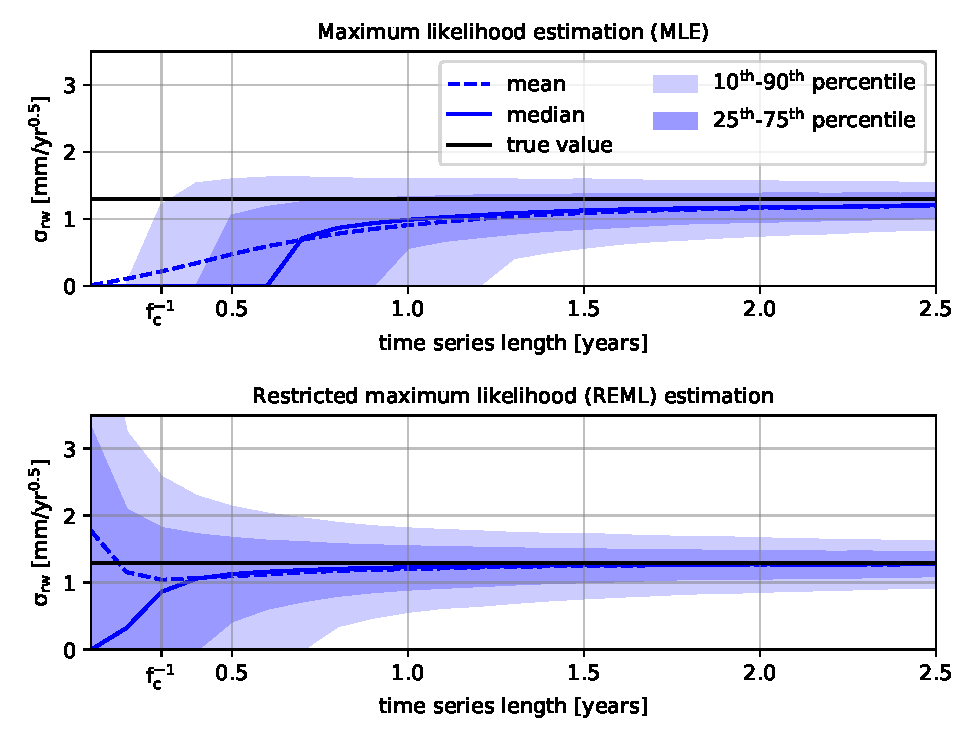
\includegraphics{figure_1.pdf}
\caption{Random walk amplitudes, $\sigma_{rw}$, estimated by the MLE and REML methods from synthetic data. The length of the synthetic time series used to estimate $\sigma_{rw}$ is varied from 0.1 yr to 2.5 yr. The black line indicates the true random walk scale ($\sigma_{rw}=1.3$), the light blue region shows the 10-90 percentile of estimates, the dark blue region shows the 25-75 percentile of estimates, the solid blue line indicates the median, and the dashed blue line indicates the mean.}   
\label{fig:1}
\end{figure*}

The distribution of $\sigma_{rw}$ estimated by the MLE method indicates that there is a bias towards underestimating $\sigma_{rw}$ when the length of the time series is comparable to $f_c^{-1}$, which is 0.3 yr in this demonstration. The bias is appreciable when the time series is shorter than ${\sim}1$ yr, and estimates of $\sigma_{rw}$ cluster around 0.0 when the time series is shorter than $f_c^{-1}$. The distribution tightens up around the true value and remains relatively constant for time series with length greater than ${\sim}1$ yr. This is consistent \citet{Langbein1997} who said that the time series should be at least 5 times greater than $f_c^{-1}$ to get a good estimate of the random walk component. However, the mean and median of the distribution tends to be slightly less than the true value even when the full length of the time series is used.

In contrast, the REML method does significantly better at estimating $\sigma_{rw}$. For every time series length considered, the true value for $\sigma_{rw}$ is within the 25-75 percentile of estimated $\sigma_{rw}$. For time series longer than $f_c^{-1}$, the mean and median of estimated $\sigma_{rw}$ closely resembles the true value, indicating that the REML method is indeed unbiased. When the length of the time series is less than $f_c^{-1}$, the mean and median deviate from the true value and the variance of estimated $\sigma_{rw}$ sharply increases. For such short time series, the random walk component cannot be resolved because it is being masked by the white noise.

\section{Discussion and conclusion}\label{sec:conclusion}
The MLE method is the most commonly used method for quantifying noise in geodetic time series, despite the fact that it is known to be biased. The bias in the MLE method can result in underestimated uncertainties in geophysical parameters derived from geodetic time series \citep{Langbein2012}. The intention of this paper is to bring the REML method to light in the geodetic community as an unbiased alternative to the MLE method. Given the widespread usage of the MLE method, it may not be realistic to suggest that researchers abandon it in favor of the REML method.  However, the REML method is nearly identical to the MLE method in terms of its computational cost and in terms of its implementation. Indeed, the only difference between the log likelihood functions being maximized by the REML and MLE methods is that the REML method includes two additional, easily computed, terms (See Appendix 1). We can therefore view the REML method as merely an unbiased correction to the MLE method.     

In this paper, we have used synthetic tests to demonstrate that the REML method does not suffer from the bias inherent in the MLE method from \citet{Langbein1997}. We also show that the REML method is able to characterize random walk noise in geodetic time series that are as short at $f_c^{-1}$. In contrast, the MLE method can only accurately quantify random walk noise for time series that are several times longer than $f_c^{-1}$. Furthermore, the MLE method and REML method have nearly identical computational costs. We believe that the REML method should always be preferred over the MLE method for quantifying noise in geodetic time series. 

\begin{acknowledgements}
%If you'd like to thank anyone, place your comments here
%and remove the percent signs.
\end{acknowledgements}

\section*{Appendix 1: REML algorithm}

Algorithm 1 demonstrates how to efficiently compute the log of the REML likelihood function. For comparison, we include Algorithm 2, which evaluates the log of the MLE likelihood function. If we assume that $m \ll n$, then the main computational burden in both algorithms is computing the Cholesky decomposition of $\mathbf{\Sigma}$. Since we are just interested in finding the $\mathbf{\Sigma}$ that maximizes these functions, we can omit the terms in the log likelihood functions that are independent of $\mathbf{\Sigma}$. In that case, the only difference between the two algorithms will be that Algorithm 1 includes a summation along the diagonals of $\mathbf{C}$ in the log likelihood function.    



\begin{algorithm}\label{alg:1}
\caption{Function that takes $\mathbf{d}$, $\mathbf{\Sigma}$, and $\mathbf{G}$ as input and returns the logarithm of eq. (\ref{eq:reml}). We use the notation $\mathbf{X} \backslash \mathbf{Z}$ to denote solving the system of equations $\mathbf{XY} = \mathbf{Z}$ for $\mathbf{Y}$.} 
\begin{algorithmic}
\Function{$reml\_log\_likelihood$}{$\mathbf{d}$,$\mathbf{\Sigma}$,$\mathbf{G}$}
\State $\mathbf{A} \gets cholesky(\mathbf{\Sigma})$ 
\State $\mathbf{B} \gets \mathbf{A} \backslash \mathbf{G}$
\State $\mathbf{C} \gets cholesky(\mathbf{B}^T\mathbf{B})$
\State $\mathbf{D} \gets cholesky(\mathbf{G}^T\mathbf{G})$
\State $\mathbf{a} \gets \mathbf{A} \backslash \mathbf{d}$
\State $\mathbf{b} \gets \mathbf{C} \backslash (\mathbf{B}^T\mathbf{a})$
\State \Return $\sum_i^m \log(D_{ii}) - 
                \sum_i^n \log(A_{ii}) - 
                \sum_i^m \log(C_{ii}) - 
                \frac{1}{2}\mathbf{a}^T\mathbf{a} + 
                \frac{1}{2}\mathbf{b}^T\mathbf{b} -
                \frac{n-m}{2}\log(2\pi)$
\EndFunction
\end{algorithmic}
\end{algorithm}

\begin{algorithm}\label{alg:2}
\caption{Function that takes $\mathbf{d}$, $\mathbf{\Sigma}$, and $\mathbf{G}$ as input and returns the logarithm of eq. (\ref{eq:mle}).} 
\begin{algorithmic}
\Function{$mle\_log\_likelihood$}{$\mathbf{d}$,$\mathbf{\Sigma}$,$\mathbf{G}$}
\State $\mathbf{A} \gets cholesky(\mathbf{\Sigma})$ 
\State $\mathbf{B} \gets \mathbf{A} \backslash \mathbf{G}$
\State $\mathbf{C} \gets cholesky(\mathbf{B}^T\mathbf{B})$
\State $\mathbf{a} \gets \mathbf{A} \backslash \mathbf{d}$
\State $\mathbf{b} \gets \mathbf{C} \backslash (\mathbf{B}^T\mathbf{a})$
\State \Return $-\sum_i^n \log(A_{ii}) - 
                \frac{1}{2}\mathbf{a}^T\mathbf{a} + 
                \frac{1}{2}\mathbf{b}^T\mathbf{b} -
                \frac{n}{2}\log(2\pi)$
\EndFunction
\end{algorithmic}
\end{algorithm}


% BibTeX users please use one of
\bibliographystyle{spbasic}      % basic style, author-year citations
%\bibliographystyle{spmpsci}      % mathematics and physical sciences
%\bibliographystyle{spphys}       % APS-like style for physics
\bibliography{mybib}   % name your BibTeX data base

\end{document}

